\section{Mode sum formula}
\label{sec:mode-sum-formula}
Vacuum polarization in \cite{ambjorn_properties_1983} is defined through a mode sum formula
\begin{align}
\begin{split}
        \rho &= \sum_{n>0}^{} \rho_n \\&= \sum_{n>0}^{}\big[(\omega_n-\varepsilon A_0)\lvert \phi_n \rvert^2
    - ( \omega_n +\varepsilon A_0) \lvert\phi_{-n}\rvert^2
    \big],
\end{split}
    \label{eq:mode-sum}    
\end{align}
so called since the total charge density is calculated as the sum of the contribution $\rho_n$ of each mode to the total charge. 
The above expression cannot be obtained from a manifestly gauge invariant renormalization scheme, and also relies on a specific pairing of the modes in the series to be convergent. 
Furthermore, in using the iterative procedure discussed in the following section,~\cite{ambjorn_properties_1983} truncated the mode sum to the first mode. Fig.~\ref{fig:hambjorn} shows the different $\rho$ resulting from the different prescriptions. At first sight, it might be surprising that a field subject to DBC has non-zero vacuum polarization at the boundaries. This is precisely due to the missing $\frac{\varepsilon^2}{\pi}A_0$ term in Eq.~\eqref{eq:mode-sum}. 
In using the iterative procedure \cite{ambjorn_properties_1983} truncates the mode sum \eqref{eq:mode-sum} to the first mode, which leads to the red curve in Fig.~\ref{fig:hambjorn}, leading to a vacuum polarization aproximately an order of magnitude stronger than the one one would obtain when using Eq.~\eqref{eq:vacuum-polarization-long}.


\begin{figure}
    \centering
    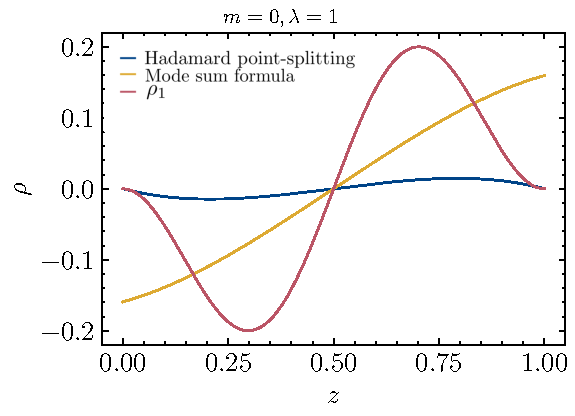
\includegraphics[width=0.45\textwidth]{Figures/dirichlet/hambjorn_annotated.pdf}
    \caption{Three different $\rho$ for the same massless scalar field subject to DBC: In blue, the correct prescription as explained in \cite{wernersson_vacuum_2021}. In orange, $\rho$ calculated through the mode sum \eqref{eq:mode-sum}. In red, $\rho$ defined through the mode sum formula, truncated to the first mode. }
    \label{fig:hambjorn}
\end{figure}